\documentclass{article}
\usepackage{listings}
\usepackage{color}
\usepackage{hyperref}
\usepackage{graphicx}
\usepackage{float}
\graphicspath{ {./src/} }


\title{Atividade Prática sobre Blockchain - Segurança e Auditoria de Sistemas}
\author{Caio Augusto de Souza Muniz, 2050889}
\date{4 de julho de 2022}


\renewcommand\lstlistingname{Quelltext}
\lstset{
    language=C,
    basicstyle=\small,
    numbers=left,
    numberstyle=\tiny,
    frame=tb,
    tabsize=2,
    columns=fixed,
    showstringspaces=false,
    showtabs=false,
    keepspaces,
    commentstyle=\color{red},
    keywordstyle=\color{blue}
}
\begin{document}
\maketitle

\section{Introdução}
A aplicação relatada neste relatório de atividade assíncrona tem como objetivos:
\begin{itemize}
\item Criação de uma aplicação de blockchain local
\item Implementação de um algoritmo de prova por trabalho local onde a dificuldade é definida pelo usuário da aplicação
\item Armazenamento os blocos validados em um arquivo
\item Implementação de rotina de verificação de integridade dos blocos.
\item O conteúdo presente nos blocos são \textit{strings}.
\end{itemize}
\section{Ferramentas}
Para o desenvolvimento da aplicação foram utilizadas as seguintes ferramentas:
\begin{itemize}
\item A linguagem escolhida foi o \textit{Javascript}, através do compilador \textit{Node.js} em sua versão 16.15;
\item Foi utilizado como base o repositório \href{https://github.com/Savjee/SavjeeCoin}{\textit{Savjee/SavjeeCoin}}, disponível no \textit{GitHub}.
\end{itemize}
\section{Metodologia}
O código-fonte da aplicação está disponível em: \href{https://github.com/caioasmuniz/local-blockchain}{\textit{caioasmuniz/local-blockchain}}

A interface da aplicação é feita pela linha de comando, esta apresenta um menu com as seguintes opções:
\subsection{Ler blockchain de um arquivo;}

\subsection{Minerar blocos pendentes;}

\begin{figure}[H]
\begin{center}
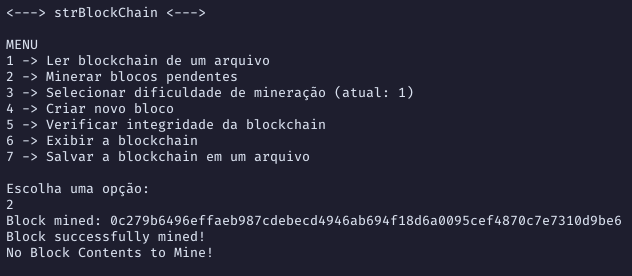
\includegraphics[scale=0.5]{mineBlock.png}
  \caption{Captura de tela da função de mineração do bloco}
\end{center}
\end{figure}

\subsection{Selecionar dificuldade de mineração;}
\begin{figure}[H]
  \begin{center}
    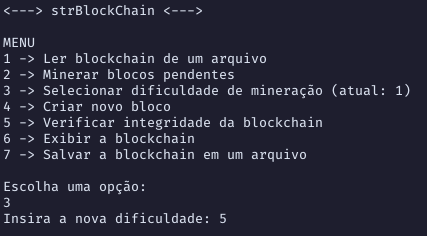
\includegraphics[scale=0.5]{selectDif.png}
    \caption{Captura de tela da função de seleção da dificuldade de mineração}
  \end{center}
\end{figure}

\subsection{Criar novo bloco;}
\begin{figure}[H]
\begin{center}
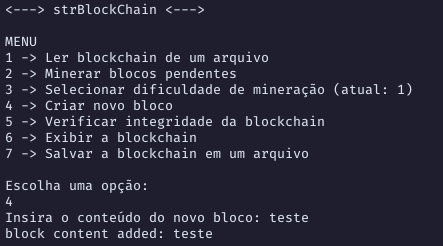
\includegraphics[scale=0.5]{insertBlock.png}
  \caption{Captura de tela da função de criação de um bloco}
\end{center}
\end{figure}

\subsection{Verificar integridade da \textit{blockchain};}
\begin{figure}[H]
  \begin{center}
    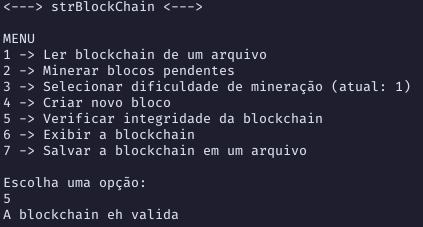
\includegraphics[scale=0.5]{verifyChain.png}
    \caption{Captura de tela da função de verificação de integridade da \textit{blockchain}}
  \end{center}
\end{figure}

\subsection{Exibir a \textit{blockchain};}

\begin{figure}[H]
\begin{center}
  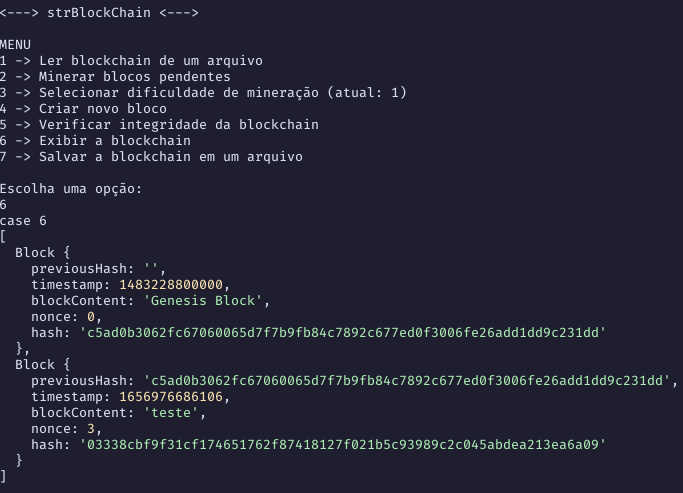
\includegraphics[scale=0.5]{showChain.png}
\end{center}\caption{Captura de tela da função exibição da \textit
  {blockchain}}
\end{figure}

\subsection{Salvar a \textit{blockchain} em um arquivo;}

\begin{figure}[H]
\begin{center}
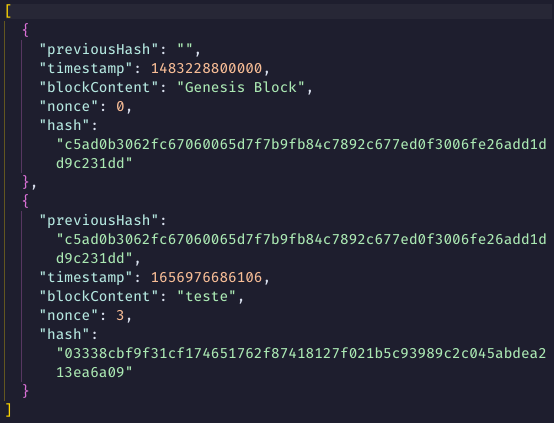
\includegraphics[scale=0.5]{outputFile.png}
  \caption{Conteúdo do arquivo contendo a \textit{blockchain}}
\end{center}
\end{figure}
\section{Análise do Impacto da Dificuldade}
Para a observação do impacto da dificuldade no tempo de execução do algoritmo, foi utilizado o \textit{script} "\textit{test-difficulty.js}", presente no \href{https://github.com/caioasmuniz/local-blockchain}{repositório da atividade}. O \textit{script} continuamente insere e minera uma quantidade de blocos na \textit{blockchain}, enquanto monitora e loga a duração de cada inserção. Este processo foi realizado para cada uma das dificuldades de 1 a 6, tendo 20 blocos gerados e minerados em cada uma das dificuldades. Após a execução do script, foi gerada a seguinte tabela com média e desvio padrão do tempo de execução:
\begin{table}[h]
  \begin{tabular}{| c | c | c |}
    \hline
    Dificuldade & Tempo Médio de execução (ms) & Desvio Padrão (ms) \\
    \hline
    1           & 0.3                          & 0.4775             \\
    \hline
    2           & 2.95                         & 3.4301             \\
    \hline
    3           & 15.4                         & 15.6277            \\
    \hline
    4           & 287.4                        & 207.9394           \\
    \hline
    5           & 4366.15                      & 4004.0907          \\
    \hline
    6           & 87177.7                      & 59671.2204         \\
    \hline
  \end{tabular}
  \caption{Tabela de tempo médio de execução e desvio padrão de acordo com a dificuldade}
\end{table}

Além disso, foi gerado o seguinte gráfico do tempo médio de mineração pela dificuldade:
\begin{figure}[h!]
  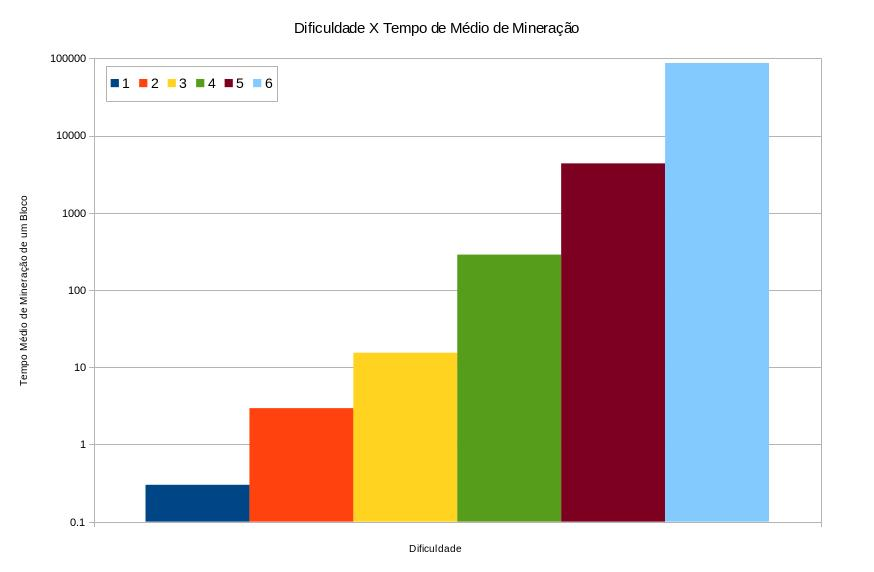
\includegraphics[width=\textwidth]{difficulty-graph.jpg}
\caption{Gráfico de Dificuldade pelo tempo de mineração}
\end{figure}

A partir dos dados coletados, é possível se observar uma relação direta entre a dificuldade de mineração de um bloco e o tempo de mineração deste. Pode-se inferir também que esta relação é exponencial, tendo em vista a escala logaritmica utilizada para a representação dos dados no gráfico.
\end{document}
